\chapter{Gugus Fungsi dan Keluarga Senyawa}\label{ch:g11:functional-groups}

Bukalah sebotol cuka, sebotol penghapus cat kuku,
sekantong permen pir, lalu berjalanlah melewati lapak penjual ikan:
empat bau, tajam, \omterm{def:g6:solutions-and-solubility:solute}{bau-pelarut} yang manis, bau buah, dan amis, dan
empat jenis \omterm{def:g7:atoms-and-molecules:molecule}{molekul} yang berbeda. Masing-masing berutang baunya, dan sebagian besar sifat
kimianya, bukan kepada kerangka karbonnya, melainkan kepada sekelompok
kecil \omterm{def:g7:atoms-and-molecules:atom}{atom} yang terpasang padanya: oksigen dan hidrogen di satu tempat,
sebuah \omterm{def:g7:atoms-and-molecules:atom}{atom} nitrogen di tempat lain. Para ahli kimia memilah \omterm{def:g11:organic-skeletons:organic}{senyawa
organik} menurut gugus-gugus ini.

\begin{recall}
\omterm{def:g11:organic-skeletons:formulas}{Rumus kerangka}, nama \omterm{def:g11:organic-skeletons:alkane}{alkana} dan \omterm{def:g11:organic-skeletons:alkane}{gugus alkil}, \omterm{def:g11:organic-skeletons:isomer}{isomer}
(\cref{ch:g11:organic-skeletons}). \omterm{def:g11:polarity-and-cohesion:polar-bond}{Ikatan polar} dan \omterm{def:g11:polarity-and-cohesion:hydrogen-bond}{ikatan hidrogen}
(\cref{ch:g11:polarity-and-cohesion}).
\end{recall}

\begin{omfigure}
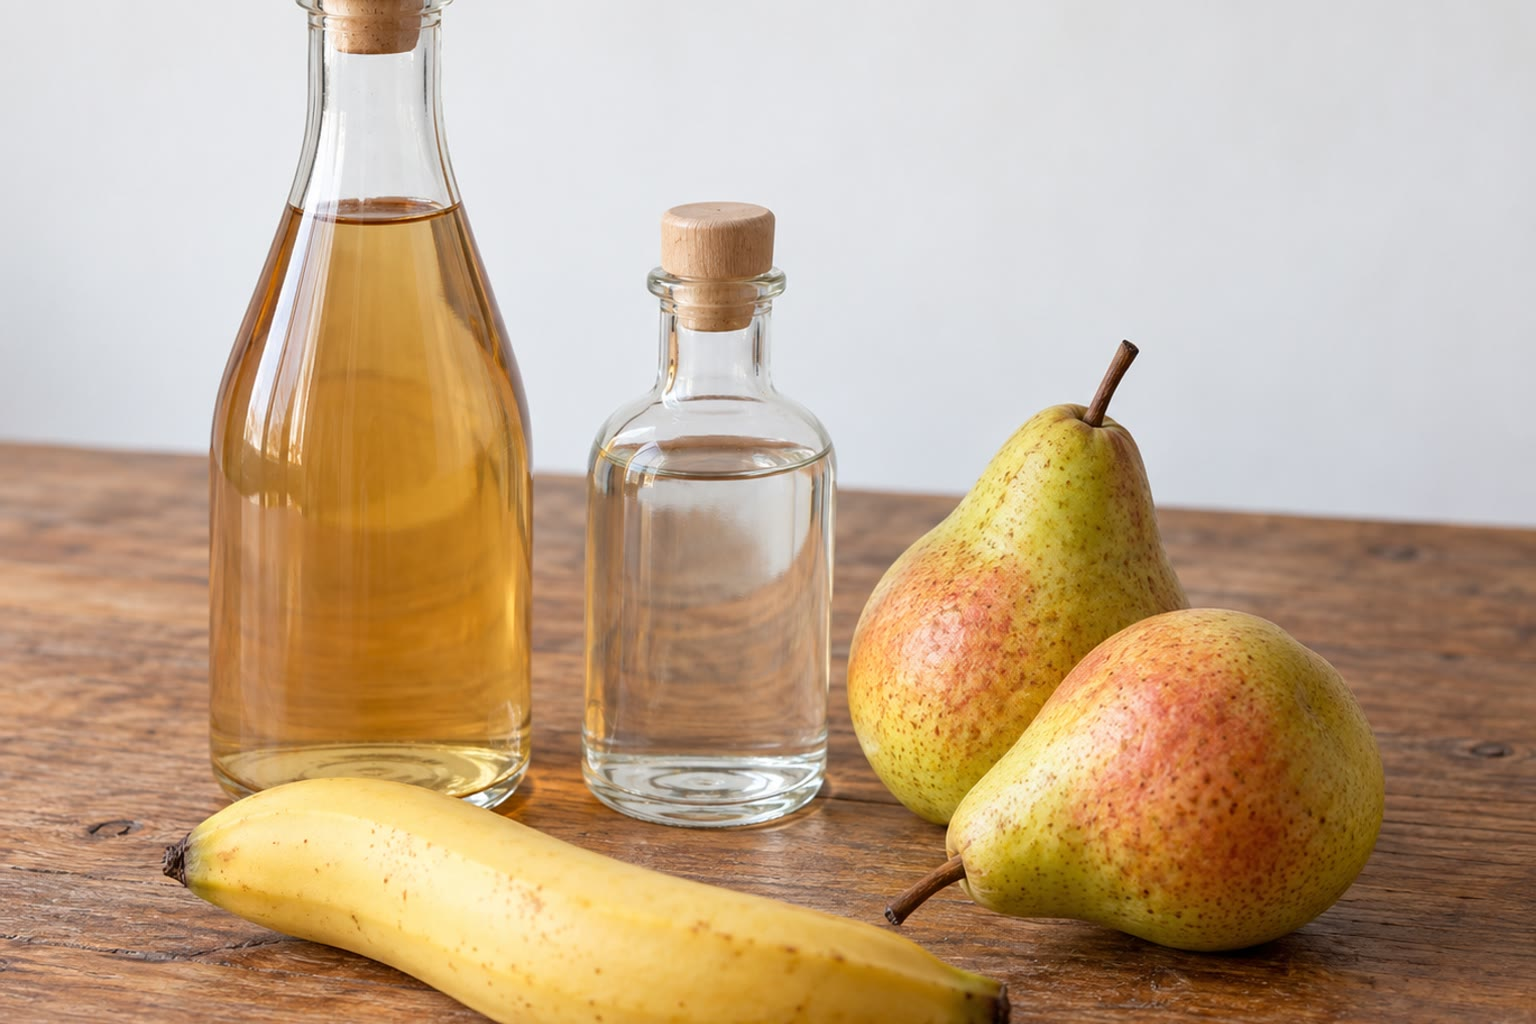
\includegraphics[width=0.5\linewidth]{images/book1/ai/g11-still-life-esters.jpg}

{\small Cuka, \omterm{def:g6:solutions-and-solubility:solute}{pelarut}, buah: setiap bau berasal dari sekelompok \omterm{def:g7:atoms-and-molecules:atom}{atom} yang
berbeda pada kerangka karbon.}
\end{omfigure}

\section{Gugus fungsi}

\begin{definition}[Gugus fungsi]\label{def:g11:functional-groups:functional-group}
Yang disebut \emph{gugus fungsi}\index{gugus fungsi} adalah sekelompok
\omterm{def:g7:atoms-and-molecules:atom}{atom}, selain \omterm{def:g7:atoms-and-molecules:atom}{atom-atom} karbon dan hidrogen kerangka yang hanya
dihubungkan oleh ikatan tunggal, yang memberi sebuah \omterm{def:g7:atoms-and-molecules:molecule}{molekul}
reaksi-reaksinya yang khas. Senyawa-senyawa yang memiliki gugus fungsi
yang sama membentuk satu keluarga.
\end{definition}

\begin{omfigure}
\renewcommand{\arraystretch}{1.35}
\footnotesize
\begin{tabular}{@{}l@{\enspace}l@{\enspace}l@{\enspace}l@{\enspace}l@{}}
\hline
gugus & rumus & keluarga & akhiran nama & contoh \\
\hline
hidroksil & \ce{-OH} & \omterm{def:g11:functional-groups:alcohol}{alkohol} & \emph{-ol} & etanol, \ce{CH3-CH2-OH} \\
karbonil (ujung) & \ce{-CHO} & \omterm{def:g11:functional-groups:carbonyl}{aldehida} & \emph{-al} & etanal, \ce{CH3-CHO} \\
karbonil (tengah) & \ce{C-CO-C} & \omterm{def:g11:functional-groups:carbonyl}{keton} & \emph{-on} & propanon, \ce{CH3-CO-CH3} \\
karboksil & \ce{-COOH} & \omterm{def:g11:functional-groups:carboxylic-acid}{asam karboksilat} & \emph{asam \ldots-oat} & asam etanoat, \ce{CH3-COOH} \\
\omterm{def:g11:functional-groups:carboxylic-acid}{ester} & \ce{C-COO-C} & \omterm{def:g11:functional-groups:carboxylic-acid}{ester} & \emph{-il \ldots-oat} & etil etanoat, \ce{CH3-COO-CH2-CH3} \\
\omterm{def:g11:functional-groups:amine}{amina} & \ce{-NH2} & \omterm{def:g11:functional-groups:amine}{amina} & \emph{-amina} & etanamina, \ce{CH3-CH2-NH2} \\
\omterm{def:g11:functional-groups:amine}{amida} & \ce{-CONH2} & \omterm{def:g11:functional-groups:amine}{amida} & \emph{-amida} & etanamida, \ce{CH3-CONH2} \\
\omterm{def:g10:electron-shells:family}{halogen} & \ce{C-X} & \omterm{def:g11:functional-groups:halogenoalkane}{haloalkana} & awalan \emph{kloro-}, \ldots & klorometana, \ce{CH3Cl} \\
\omterm{def:g10:lewis-and-shape:multiple-bond}{ikatan rangkap} & \ce{C=C} & \omterm{def:g11:functional-groups:halogenoalkane}{alkena} & \emph{-ena} & etena, \ce{CH2=CH2} \\
\hline
\end{tabular}\par\medskip

\setchemfig{atom sep=1.4em}
\begin{tabular}{@{}c@{\quad}c@{\quad}c@{\quad}c@{\quad}c@{}}
\chemfig{R-C(=[2]O)-H} & \chemfig{R-C(=[2]O)-R'} & \chemfig{R-C(=[2]O)-O-H} &
\chemfig{R-C(=[2]O)-O-R'} & \chemfig{R-C(=[2]O)-N(-[1]H)-[7]H} \\
\small \omterm{def:g11:functional-groups:carbonyl}{aldehida} & \small \omterm{def:g11:functional-groups:carbonyl}{keton} & \small \omterm{def:g11:functional-groups:carboxylic-acid}{asam karboksilat} & \small \omterm{def:g11:functional-groups:carboxylic-acid}{ester} &
\small \omterm{def:g11:functional-groups:amine}{amida}
\end{tabular}\par\medskip

{\small Gugus-gugus fungsi utama, dan kelima gugus yang dibangun di atas
gugus karbonil \ce{C=O}, digambar lengkap. R dan R$'$ menyatakan rantai
karbon (\omterm{def:g11:organic-skeletons:alkane}{gugus alkil}) dan X sebuah \omterm{def:g7:atoms-and-molecules:atom}{atom} \omterm{def:g10:electron-shells:family}{halogen} (F, Cl, Br, I).}
\end{omfigure}

\section{Alkohol dan kelasnya}

\begin{definition}[Alkohol, kelas alkohol]\label{def:g11:functional-groups:alcohol}
Sebuah \emph{alkohol}\index{alkohol} memiliki gugus hidroksil \ce{-OH}
yang terikat pada \omterm{def:g7:atoms-and-molecules:atom}{atom} karbon yang hanya memiliki ikatan tunggal. Yang
disebut \emph{kelas alkohol}\index{kelas alkohol} adalah primer,
sekunder, atau tersier, menurut apakah \omterm{def:g7:atoms-and-molecules:atom}{atom} karbon yang mengikat
\ce{-OH} terikat pada satu, dua, atau tiga \omterm{def:g7:atoms-and-molecules:atom}{atom} karbon lain. (Metanol,
\ce{CH3OH}, yang karbonnya tidak terikat pada karbon lain, digolongkan
bersama alkohol primer.)
\end{definition}

\begin{omfigure}
\setchemfig{atom sep=1.9em}
\begin{tabular}{ccc}
\chemfig{-[:30]-[:-30]-[:30]-[:-30]OH} &
\chemfig{-[:30](-[:90]OH)-[:-30]-[:30]} &
\chemfig{-[:0](-[:90]OH)(-[:-90])-[:0]} \\[4pt]
\small butan-1-ol & \small butan-2-ol & \small 2-metilpropan-2-ol \\
\small \textbf{primer} & \small \textbf{sekunder} & \small \textbf{tersier} \\
\small (C pada \ce{-OH}: 1 tetangga karbon) & \small (2 tetangga) &
\small (3 tetangga)
\end{tabular}

{\small Tiga \omterm{def:g11:organic-skeletons:isomer}{isomer} \ce{C4H10O}, tiga \omterm{def:g11:functional-groups:alcohol}{kelas alkohol}.}
\end{omfigure}

\section{Aldehida, keton, asam, dan ester}

\begin{definition}[Aldehida, keton]\label{def:g11:functional-groups:carbonyl}
Gugus karbonil adalah \omterm{def:g10:lewis-and-shape:multiple-bond}{ikatan rangkap} \ce{C=O}. Jika \omterm{def:g7:atoms-and-molecules:atom}{atom} karbonnya
berada di ujung rantai (terikat pada sedikitnya satu \omterm{def:g7:atoms-and-molecules:atom}{atom} hidrogen),
senyawanya adalah \emph{aldehida}\index{aldehida}; jika berada di tengah
rantai (terikat pada dua \omterm{def:g7:atoms-and-molecules:atom}{atom} karbon), senyawanya adalah
\emph{keton}\index{keton}.
\end{definition}

\begin{definition}[Asam karboksilat, ester]\label{def:g11:functional-groups:carboxylic-acid}
Sebuah \emph{asam karboksilat}\index{asam karboksilat} memiliki gugus
karboksil \ce{-COOH}, yaitu karbonil dan hidroksil pada \omterm{def:g7:atoms-and-molecules:atom}{atom} karbon
yang sama. Sebuah \emph{ester}\index{ester} memiliki gugus \ce{-COO-} di
antara dua rantai karbon: ester berkerabat dengan sebuah asam, yang
\ce{-OH}-nya telah diganti dengan \ce{-O-}R$'$ yang berasal dari sebuah
\omterm{def:g11:functional-groups:alcohol}{alkohol}.
\end{definition}

\begin{example}[Etil etanoat]\label{ex:g11:functional-groups:ethyl-ethanoate}
\omterm{def:g6:solutions-and-solubility:solute}{Pelarut} etil etanoat, \ce{CH3-COO-CH2-CH3}, berbau permen pir dan
penghapus cat kuku. ``Bagian asam''-nya, \ce{CH3-CO}, berasal dari asam
etanoat \ce{CH3-COOH} dan memberikan kata kedua nama itu,
\emph{etanoat}; ``bagian \omterm{def:g11:functional-groups:alcohol}{alkohol}''-nya, \ce{O-CH2-CH3}, berasal dari
etanol \ce{CH3-CH2-OH} dan memberikan kata pertama, \emph{etil}. Sebuah
bab berikutnya menunjukkan cara membuat \omterm{def:g11:functional-groups:carboxylic-acid}{ester} dari asam dan \omterm{def:g11:functional-groups:alcohol}{alkoholnya}.
\end{example}

\begin{omfigure}
\setchemfig{atom sep=2.2em}
\chemfig{@{a}H_3C-@{c}C(=[2]@{o}O)-@{x}O-CH_2-@{z}CH_3}
\chemmove{
  \fill[omProp, opacity=0.14, rounded corners]
    ($(a.south west)+(-0.12,-0.15)$) rectangle ($(o.north east)+(0.25,0.12)$);
  \fill[omDef, opacity=0.14, rounded corners]
    ($(x.south west)+(-0.2,-0.15)$) rectangle ($(z.north east)+(0.4,0.75)$);
  \node[omProp, anchor=north east, align=right, font=\small] at ($(c.south)+(0.15,-0.25)$)
    {bagian asam, dari asam etanoat:\\ \emph{etanoat}};
  \node[omDef, anchor=north west, align=left, font=\small] at ($(x.south)+(0.05,-0.25)$)
    {bagian alkohol, dari etanol:\\ \emph{etil}};}
\par\vspace{1.4cm}

{\small Menamai \omterm{def:g11:functional-groups:carboxylic-acid}{ester}: bagian \omterm{def:g11:functional-groups:alcohol}{alkohol} memberikan nama alkil
(\emph{etil}), bagian asam memberikan akhiran \emph{-oat}
(\emph{etanoat}); namanya ``etil etanoat''.}
\end{omfigure}

\section{Amina, amida, haloalkana, dan alkena}


\begin{definition}[Amina, amida]\label{def:g11:functional-groups:amine}
Sebuah \emph{amina}\index{amina} memiliki \omterm{def:g7:atoms-and-molecules:atom}{atom} nitrogen yang terikat pada
rantai karbon dengan ikatan tunggal, seperti pada \ce{-NH2}. Sebuah
\emph{amida}\index{amida} memiliki \omterm{def:g7:atoms-and-molecules:atom}{atom} nitrogen yang terikat pada karbon
gugus karbonil, seperti pada \ce{-CO-NH2}.
\end{definition}

\begin{definition}[Haloalkana, alkena]\label{def:g11:functional-groups:halogenoalkane}
Sebuah \emph{haloalkana}\index{haloalkana} adalah \omterm{def:g11:organic-skeletons:alkane}{alkana} yang satu atau
lebih \omterm{def:g7:atoms-and-molecules:atom}{atom} hidrogennya diganti dengan \omterm{def:g7:atoms-and-molecules:atom}{atom} \omterm{def:g10:electron-shells:family}{halogen} (F, Cl, Br, I).
Sebuah \emph{alkena}\index{alkena} memiliki \omterm{def:g10:lewis-and-shape:multiple-bond}{ikatan rangkap}
karbon--karbon, \ce{C=C}.
\end{definition}

\begin{remark}[Bau dan gugus]\label{rem:g11:functional-groups:smells}
Banyak \omterm{def:g11:functional-groups:amine}{amina} kecil berbau ikan busuk, dan bau ikan yang sudah tidak
segar sebagian besar disebabkan oleh \omterm{def:g11:functional-groups:amine}{amina}. Banyak \omterm{def:g11:functional-groups:carboxylic-acid}{ester} kecil berbau
buah. \omterm{def:g11:functional-groups:carboxylic-acid}{Asam karboksilat} kecil berbau tajam, seperti cuka; propanon,
sebuah \omterm{def:g11:functional-groups:carbonyl}{keton}, adalah bau \omterm{def:g6:solutions-and-solubility:solute}{pelarut} yang akrab dari penghapus cat kuku.
\end{remark}

\section{Tata nama}

\begin{method}[Menamai senyawa organik dengan satu gugus fungsi]\label{met:g11:functional-groups:naming}
\begin{enumerate}
  \item Carilah rantai karbon terpanjang yang \emph{memuat} karbon \omterm{def:g11:functional-groups:functional-group}{gugus
        fungsinya} (atau, untuk \omterm{def:g11:functional-groups:alcohol}{alkohol} dan \omterm{def:g11:functional-groups:amine}{amina}, karbon yang
        mengikatnya): rantai itu memberikan nama induknya.
  \item Nomorilah rantai itu dari ujung yang memberikan nomor terkecil
        kepada \omterm{def:g11:functional-groups:functional-group}{gugus fungsinya}.
  \item Ganti akhiran \emph{-a} \omterm{def:g11:organic-skeletons:alkane}{alkana} dengan akhiran keluarga itu,
        didahului letak gugusnya jika perlu: propan-2-ol, butan-2-on.
        (\omterm{def:g11:functional-groups:carbonyl}{Aldehida}, asam, dan \omterm{def:g11:functional-groups:amine}{amida} memiliki gugusnya pada karbon 1:
        tanpa nomor.)
  \item Tambahkan substituen-substituen alkil sebagai awalan, beserta
        letaknya, seperti pada \omterm{def:g11:organic-skeletons:alkane}{alkana}; \omterm{def:g10:electron-shells:family}{halogen} selalu menjadi awalan
        (2-kloropropana).
\end{enumerate}
\end{method}

\begin{example}[Empat nama]\label{ex:g11:functional-groups:names}
\setchemfig{atom sep=1.7em}
\chemfig{-[:30](-[:90]OH)-[:-30]} adalah propan-2-ol (\omterm{def:g11:functional-groups:alcohol}{alkohol} sekunder);
\chemfig{-[:30](=[:90]O)-[:-30]-[:30]} adalah butan-2-on;
\chemfig{-[:30]-[:-30]-[:30](=[:90]O)-[:-30]OH} adalah asam butanoat;
\chemfig{-[:30](-[:90])-[:-30]-[:30]=[:-30]O} adalah 3-metilbutanal.
\end{example}

\begin{omfigure}
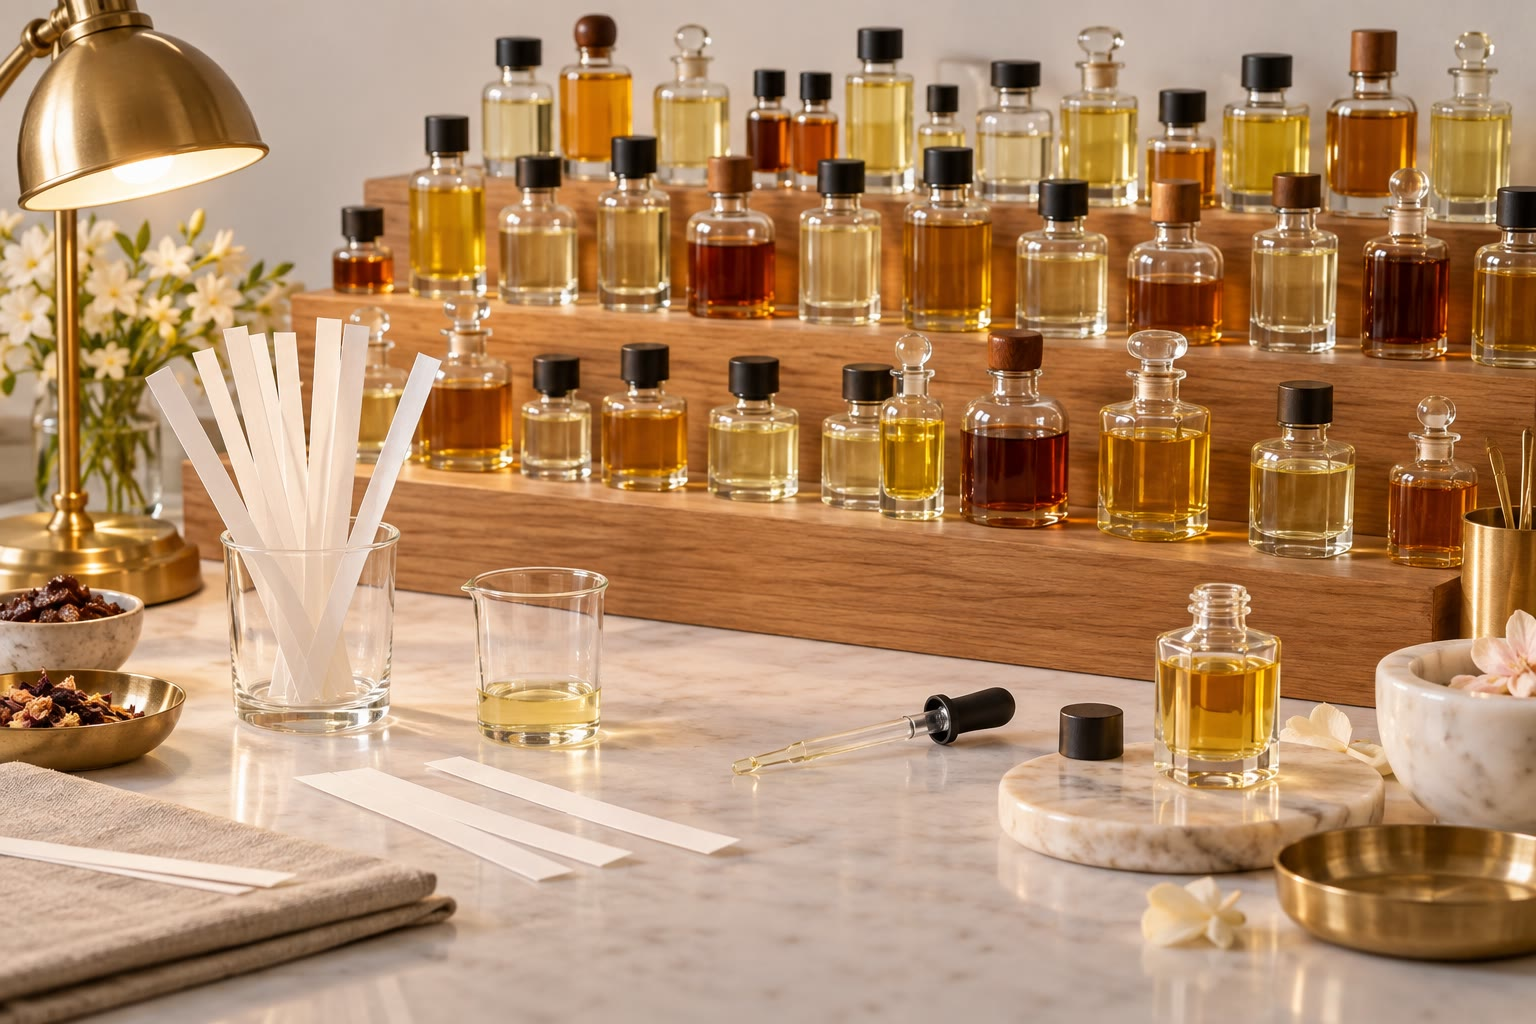
\includegraphics[width=0.48\linewidth]{images/book1/ai/g11-perfumer-lab.jpg}

{\small Meja kerja seorang peracik parfum: banyak botolnya berisi \omterm{def:g11:functional-groups:carboxylic-acid}{ester},
\omterm{def:g11:functional-groups:alcohol}{alkohol}, \omterm{def:g11:functional-groups:carbonyl}{aldehida}, dan \omterm{def:g11:functional-groups:carbonyl}{keton}.}
\end{omfigure}

\begin{safety}{\ghs[0.82cm]{GHS02}\ghs[0.82cm]{GHS05}\ghs[0.82cm]{GHS07}}
% ledger: ghs:acetone, ghs:acetic-acid
Propanon sangat mudah menyala dan menyebabkan iritasi mata; uapnya
menimbulkan kantuk. Asam etanoat murni mudah menyala dan menyebabkan luka
bakar parah pada kulit dan mata; cuka adalah larutan encernya. Bau tidak
pernah diuji dengan mengendus labu: uapnya dikibaskan perlahan ke arah
hidung dengan tangan, dan hanya jika guru mengizinkan.
\end{safety}

\section{Latihan}


\begin{exercise}[$\star$]\label{exo:g11:functional-groups:1}
Sebutkan \omterm{def:g11:functional-groups:functional-group}{gugus fungsi} dan keluarga setiap senyawa berikut:
\ce{CH3-CH2-CH2-OH}; \ce{CH3-CO-CH2-CH3}; \ce{CH3-CH2-COOH};
\ce{CH3-COO-CH3}; \ce{CH3-CH2-NH2}.
\end{exercise}

\begin{exercise}[$\star$]\label{exo:g11:functional-groups:2}
Namailah: \ce{CH3-OH}; \ce{CH3-CH2-CH2-OH}; \ce{HCOOH}; \ce{CH3-CH2-CHO};
\ce{CH3-CO-CH3}.
\end{exercise}

\begin{exercise}[$\star$]\label{exo:g11:functional-groups:3}
Termasuk keluarga apa setiap senyawa berikut: butan-2-ol, pentanal,
metil propanoat, propanamida, 2-bromopropana, but-1-ena?
\end{exercise}

\begin{exercise}[$\star$]\label{exo:g11:functional-groups:4}
Tuliskan \omterm{def:g11:organic-skeletons:formulas}{rumus struktur ringkas} propanal dan propanon. Manakah yang
\omterm{def:g11:functional-groups:carbonyl}{aldehida}? Bagaimana kamu mengetahuinya?
\end{exercise}

\begin{exercise}[$\star$]\label{exo:g11:functional-groups:5}
Tentukan kelas propan-1-ol, propan-2-ol, dan 2-metilpropan-2-ol.
\end{exercise}

\begin{exercise}[$\star\star$]\label{exo:g11:functional-groups:6}
Gambarlah \omterm{def:g11:organic-skeletons:formulas}{rumus kerangka} pentan-3-ol, asam 2-metilbutanoat,
heksan-2-on, dan propil etanoat.
\end{exercise}

\begin{exercise}[$\star\star$]\label{exo:g11:functional-groups:7}
Propanal dan propanon memiliki \omterm{def:g11:organic-skeletons:formulas}{rumus molekul} yang sama. Tuliskan rumus
itu. Apakah keduanya \omterm{def:g11:organic-skeletons:isomer}{isomer}? Apakah \omterm{def:g11:functional-groups:functional-group}{gugus fungsinya} sama?
\end{exercise}

\begin{exercise}[$\star\star$]\label{exo:g11:functional-groups:8}
Tuliskan \omterm{def:g11:organic-skeletons:formulas}{rumus struktur ringkas} dan nama \omterm{def:g11:functional-groups:carboxylic-acid}{ester} yang bagian asamnya
berasal dari asam metanoat \ce{HCOOH} dan bagian \omterm{def:g11:functional-groups:alcohol}{alkoholnya} dari etanol;
lalu \omterm{def:g11:functional-groups:carboxylic-acid}{ester} dari asam etanoat dan propan-1-ol.
\end{exercise}

\begin{exercise}[$\star\star$]\label{exo:g11:functional-groups:9}
Namailah \omterm{def:g11:functional-groups:carboxylic-acid}{ester-ester} \ce{CH3-COO-CH3}, \ce{CH3-CH2-COO-CH2-CH3}, dan
\ce{HCOO-CH3}, lalu sebutkan asam dan \omterm{def:g11:functional-groups:alcohol}{alkohol} kerabat masing-masing.
\end{exercise}

\begin{exercise}[$\star\star$]\label{exo:g11:functional-groups:10}
Gambarlah dan namailah keempat \omterm{def:g11:functional-groups:alcohol}{alkohol} dengan rumus \ce{C4H10O}, lalu
tentukan kelas masing-masing.
\end{exercise}

\begin{exercise}[$\star\star$]\label{exo:g11:functional-groups:11}
Dengan tabel gugus: termasuk keluarga apa \ce{CH3-CO-NH2}? Akhiran apa
yang dipakai nama \omterm{def:g11:functional-groups:halogenoalkane}{alkena}? Keluarga mana yang memiliki gugus karbonil
dengan \omterm{def:g7:atoms-and-molecules:atom}{atom} oksigen atau nitrogen pada karbon yang sama?
\end{exercise}

\begin{exercise}[$\star\star\star$]\label{exo:g11:functional-groups:12}
Lingkarilah dan namailah gugus-gugus fungsi aspirin dan parasetamol.
(Gugus \ce{-OH} yang terikat langsung pada cincin seperti pada
parasetamol disebut gugus fenol; perilakunya berbeda dari \omterm{def:g11:functional-groups:alcohol}{alkohol}.)
\begin{center}
\setchemfig{atom sep=1.6em}
\chemfig{*6(-=-(-COOH)=(-O-[:150]C(=[:90]O)-[:210]H_3C)-=)}
\qquad
\chemfig{*6((-OH)=-=(-N(-[2]H)-[7]C(=[6]O)-[1]CH_3)-=-)}
\\[2pt] \small aspirin \hspace{4.2cm} parasetamol
\end{center}
\end{exercise}

\begin{exercise}[$\star\star\star$]\label{exo:g11:functional-groups:13}
% ledger: bp:C2H5OH, bp:CH3OCH3
Etanol \ce{CH3-CH2-OH} dan metoksimetana \ce{CH3-O-CH3} memiliki \omterm{def:g11:organic-skeletons:formulas}{rumus
molekul} yang sama. Tuliskan rumus itu. Metoksimetana termasuk keluarga
yang tidak ada dalam tabel, yaitu eter. Manakah di antara keduanya yang
dapat membentuk \omterm{def:g11:polarity-and-cohesion:hydrogen-bond}{ikatan hidrogen} di antara \omterm{def:g7:atoms-and-molecules:molecule}{molekul-molekulnya} sendiri?
Manakah yang mendidih lebih tinggi (yang satu mendidih pada
\qty{78}{\celsius}, yang lain pada \qty{-25}{\celsius})?
\end{exercise}

\begin{exercise}[$\star\star\star$]\label{exo:g11:functional-groups:14}
Asam laktat, yang dihasilkan otot yang lelah, adalah
\chemfig{CH_3-CH(-[2]OH)-COOH}. Sebutkan kedua \omterm{def:g11:functional-groups:functional-group}{gugus fungsinya}. Jika
sebuah \omterm{def:g7:atoms-and-molecules:molecule}{molekul} memiliki gugus asam dan gugus lain, gugus asamnya yang
memberikan akhiran dan gugus lainnya menjadi awalan (\emph{hidroksi-}
untuk \ce{-OH}, \emph{amino-} untuk \ce{-NH2}). Namailah asam laktat,
lalu glisina, \ce{H2N-CH2-COOH}.
\end{exercise}

\begin{exercise}[$\star\star\star$]\label{exo:g11:functional-groups:15}
Anggur yang dibiarkan terbuka di \omterm{def:g4:air-a-mixture-of-gases:air}{udara} berubah menjadi cuka: etanol
menjadi asam etanoat, melalui etanal. Tuliskan \omterm{def:g11:organic-skeletons:formulas}{rumus struktur ringkas}
dan \omterm{def:g11:organic-skeletons:formulas}{rumus molekul} ketiga senyawa itu beserta keluarganya. Apa yang
berubah dalam rumus pada setiap langkah?
\end{exercise}

\section{Soal: Perisa Buah}

\begin{problem}[{Soal akhir pekan --- seorang ahli kimia perisa meracik bau
pisang: berapa massa molar molekul kuncinya?}]
\label{pb:g11:functional-groups:1}
% ledger: aw:C, aw:H, aw:O
Seorang ahli kimia perisa memiliki lima senyawa di meja kerjanya:
\begin{center}
\begin{tabular}{ll}
A & \chemfig{CH_3-C(=[2]O)-O-CH_2-CH_2-CH(-[2]CH_3)-CH_3} \\[16pt]
B & \chemfig{HO-CH_2-CH_2-CH(-[2]CH_3)-CH_3} \\[10pt]
C & \ce{CH3-COOH} \\
D & \ce{CH3-CH2-CH2-CH2-CH2-CHO} \\
E & \ce{CH3-CH2-CH2-COO-CH2-CH3}
\end{tabular}
\end{center}
A berbau pisang dan permen pir, B berbau malt, C berbau cuka, D berbau
rumput yang baru dipotong, E berbau nanas.

\medskip
\noindent\textbf{Bagian I --- Gugus dan keluarga.}
\begin{enumerate}
  \item Sebutkan \omterm{def:g11:functional-groups:functional-group}{gugus fungsi} setiap senyawa.
  \item Sebutkan keluarga masing-masing.
  \item Senyawa mana yang \omterm{def:g11:functional-groups:carboxylic-acid}{ester}? Bau apa yang dimilikinya?
  \item Apa \omterm{def:g11:functional-groups:alcohol}{kelas alkohol} B?
  \item Tuliskan \omterm{def:g11:organic-skeletons:formulas}{rumus molekul} D, lalu gambarlah sebuah \omterm{def:g11:organic-skeletons:isomer}{isomer} D yang
        berupa \omterm{def:g11:functional-groups:carbonyl}{keton}.
\end{enumerate}

\medskip
\noindent\textbf{Bagian II --- Nama-namanya.}
\begin{enumerate}[resume]
  \item Namailah B (carilah rantai terpanjang yang memuat karbon yang
        mengikat \ce{-OH}).
  \item Namailah C dan D.
  \item Namailah E, lalu sebutkan asam dan \omterm{def:g11:functional-groups:alcohol}{alkohol} kerabatnya.
  \item Jelaskan nama A, 3-metilbutil etanoat: bagian mana yang berasal
        dari asam, mana yang dari \omterm{def:g11:functional-groups:alcohol}{alkohol}?
\end{enumerate}

\medskip
\noindent\textbf{Bagian III --- Dari sebuah asam dan sebuah \omterm{def:g11:functional-groups:alcohol}{alkohol}.}
\begin{enumerate}[resume]
  \item Dengan dua senyawa mana di meja itu A berkerabat?
  \item Tuliskan \omterm{def:g11:organic-skeletons:formulas}{rumus molekul} A, B, dan C.
  \item \omterm{def:g11:functional-groups:carboxylic-acid}{Ester} dibuat dari asam dan \omterm{def:g11:functional-groups:alcohol}{alkoholnya} dengan melepaskan satu
        \omterm{def:g7:atoms-and-molecules:molecule}{molekul} kecil. Dengan rumus-rumus itu, tentukan \omterm{def:g7:atoms-and-molecules:molecule}{molekul} apa.
  \item Tuliskan persamaan pembentukan A, dalam \omterm{def:g11:organic-skeletons:formulas}{rumus molekul}, lalu
        periksalah bahwa persamaan itu setara.
\end{enumerate}

\medskip
\noindent\textbf{Bagian IV --- \omterm{def:g10:the-mole:molar-mass}{Massa molar}.}
\begin{enumerate}[resume]
  \item Hitung \omterm{def:g10:the-mole:molar-mass}{massa molar} B dan C.
  \item Simpulkan \omterm{def:g10:the-mole:molar-mass}{massa molar} A dari persamaan pada soal 13.
  \item Hitung \omterm{def:g10:the-mole:molar-mass}{massa molar} A langsung dari rumusnya, lalu bandingkan.
  \item Sebuah sampel beraroma buah yang tidak diketahui ternyata
        memiliki \omterm{def:g10:the-mole:molar-mass}{massa molar} mendekati \qty{116}{g/mol}. Apakah sampel itu
        A atau E?
  \item Asam heptanoat, \ce{CH3-(CH2)5-COOH}, berbau tengik. Tunjukkan
        bahwa senyawa itu \omterm{def:g11:organic-skeletons:isomer}{isomer} A. Dapatkah \omterm{def:g10:the-mole:molar-mass}{massa molar} saja mengenali
        sebuah senyawa?
  \item Mengapa para ahli kimia mengatakan bahwa bau itu milik \omterm{def:g11:functional-groups:functional-group}{gugus
        fungsinya} sama halnya dengan milik kerangkanya? Pakailah A dan
        asam heptanoat.
  \item Nyatakan jawaban akhirnya: berapa \omterm{def:g10:the-mole:molar-mass}{massa molar} \omterm{def:g11:functional-groups:carboxylic-acid}{ester} pisang,
        3-metilbutil etanoat?
\end{enumerate}
\end{problem}
